\documentclass{beamer}

%%%%%%%%%%%%%Solarized Theme%%%%%%%%%%%%%%%
\usecolortheme[dark,accent=cyan]{solarized}
\beamertemplatenavigationsymbolsempty
%%%%%Packages%%%%%
\usefonttheme{serif}
\usepackage[T1]{fontenc}
\usepackage[utf8]{inputenc}
\usepackage[english]{babel}
\usepackage{fontawesome}
\usepackage{minted}
\usepackage{soul}
\usepackage{ulem}

\definecolor{DarkGray}{gray}{0.1}
\usemintedstyle{paraiso-dark}


\usepackage{graphicx}
\usepackage{hyperref}
\usepackage{colortbl, xcolor}
\usepackage{booktabs}
\usepackage{amsmath,amsthm, amssymb, latexsym}

\usepackage{tikz}
\usepackage{xcolor}
\usepackage{graphicx,multirow}
\definecolor{plain}{rgb}{93,93,93}
\usetikzlibrary{positioning,arrows}
\definecolor{applegreen}{rgb}{0.55, 0.71, 0.0}
\usetikzlibrary{decorations.pathreplacing, backgrounds, fit}
\usetikzlibrary{calc,matrix}

\tikzstyle{background}=[solarizedRed, rectangle, draw, inner sep=1mm, thick,
           rounded corners=2mm]

\usepackage{standalone}
\usepackage{siunitx}

\begin{document}

\begin{frame}
    \begin{center}
        \Large{\textcolor{orange}{AQUAVIT}} \\

        \vspace{1cm}
        \normalsize{@NikoletaGlyn}

    \end{center}
\end{frame}

\begin{frame}
    \begin{center}
    
\includegraphics[width=0.24\textwidth]{static/mpi.jpg}\hspace{8pt}
    
\includegraphics[width=0.24\textwidth]{static/cardiff_uni_logo.jpg}\vspace{8pt}

    
\includegraphics[width=0.24\textwidth]{static/ssi-logo.png}\hspace{8pt}
    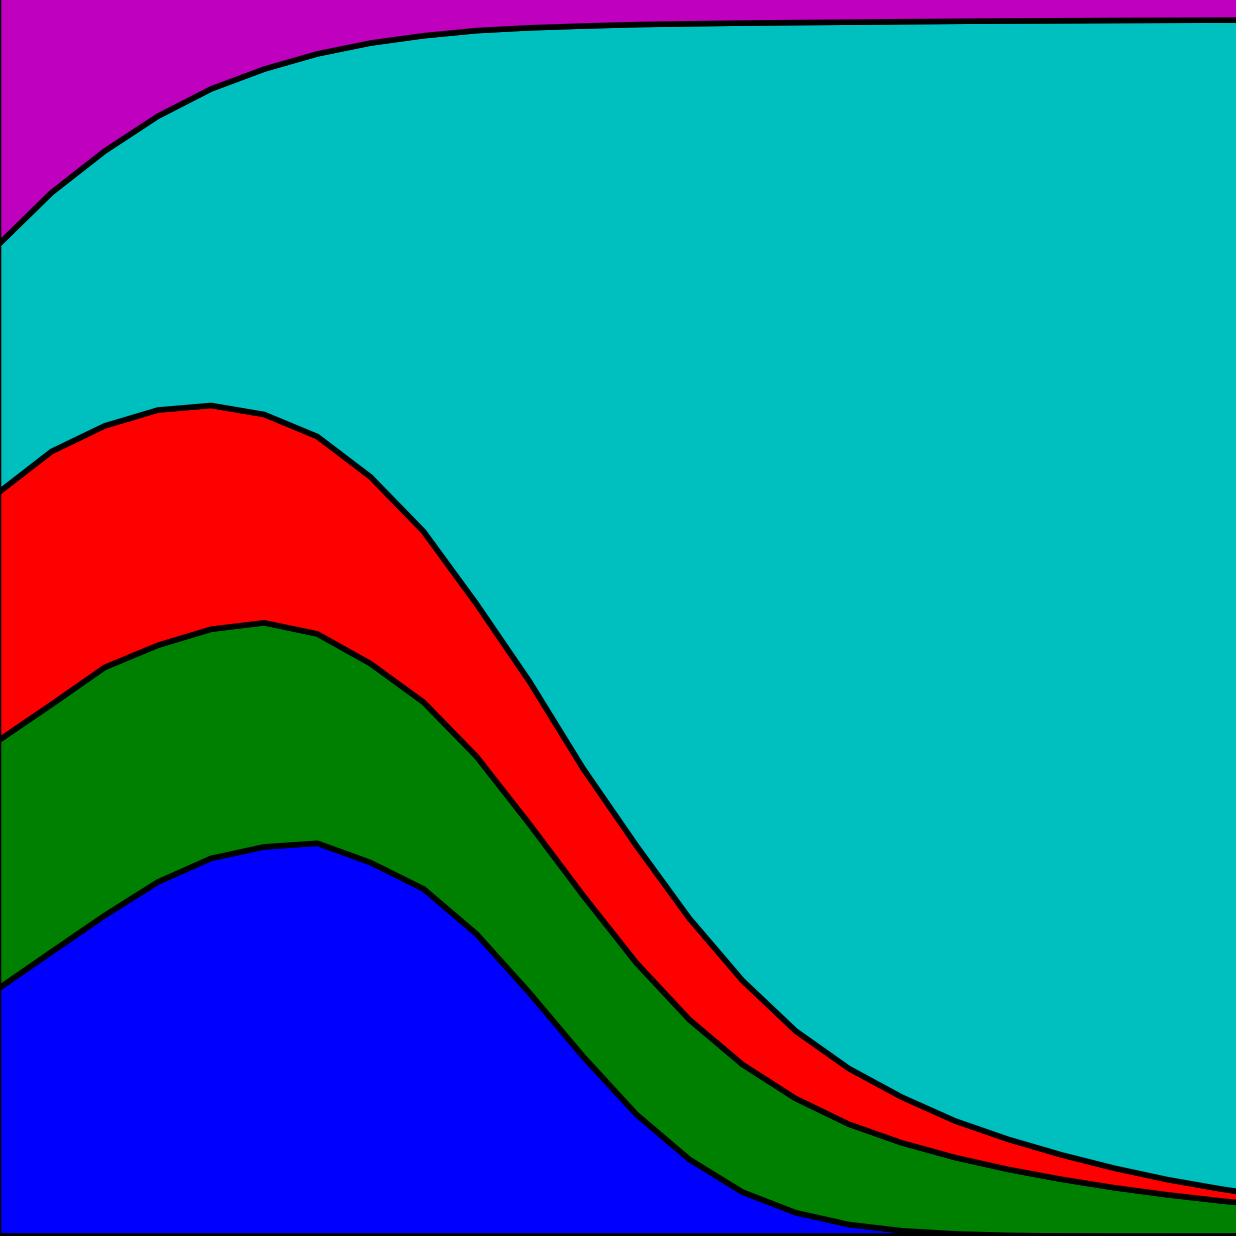
\includegraphics[width=0.24\textwidth]{static/axelrod-logo.png}
    \end{center}
\end{frame}

\begin{frame}
    \centering
    \includestandalone[width=.75\textwidth]{static/game}
\end{frame}


\begin{frame}
    \begin{center}
    \huge{
        \begin{equation*}
            \begin{pmatrix}
                (b - c, b - c) & (c, b) \\[6pt]
                (b, c) & (0, 0)
            \end{pmatrix}
        \end{equation*}}
    \end{center}
\end{frame}

\begin{frame}
    \begin{center}
    \huge{
        \begin{equation*}
            \begin{pmatrix}
                (2, \phantom{-}2) & (-1, 3) \\[6pt]
                (3, -1) & (\phantom{-}0, 0)
            \end{pmatrix}
        \end{equation*}}
    \end{center}
\end{frame}

\begin{frame}
    \begin{center}
\includestandalone[width=\textwidth]{static/iterated_prisoners_dilemma}
    \end{center}
\end{frame}

\begin{frame}
    \centering
    \includestandalone[width=.65\textwidth]{static/population}
\end{frame}

\begin{frame}
    \centering
    \includestandalone[width=.65\textwidth]{static/population_c}
\end{frame}

\begin{frame}
    \centering
    \includestandalone[width=.65\textwidth]{static/population_d}
\end{frame}

\begin{frame}
    \centering
    \includestandalone[width=.65\textwidth]{static/reactive}
\end{frame}

\begin{frame}
    \begin{center}
        \small
    \#ChooseToChallenge \\
    \faTwitter \ @NikoletaGlyn \\
    \faTwitter \ @AxelrodPython \\
    
    \vspace{1cm}
    \end{center}

    \footnotesize
    \faGithub \ \url{https://github.com/Axelrod-Python/Axelrod} \\
    $\bullet$ \url{https://axelrod.readthedocs.io/} \\
    $\bullet$ \url{https://axelrod.readthedocs.io/en/latest/tutorials/contributing/index.html} \\

    \faGithub  \ \url{https://github.com/drvinceknight} \\
    \faGithub  \ \url{https://github.com/gaffney2010} \\
    \faGithub  \ \url{https://github.com/marcharper} \\
    \faGithub  \ \url{https://github.com/meatballs} \\
\end{frame}

\end{document}